Для получения информации об атомном облаке в МОЛ использовалась схема изображенная на рис. \ref{fig:exp_photo}. 

\begin{figure}[ht]
    \centering
    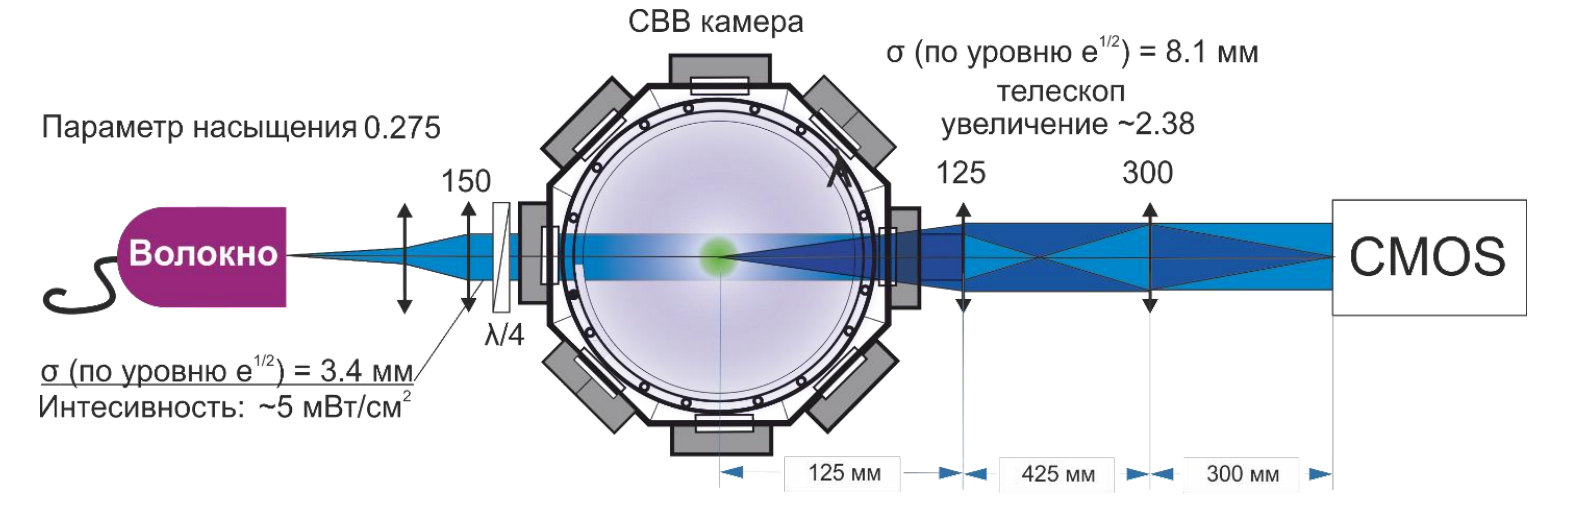
\includegraphics[width=0.9\textwidth]{figs/detect.png}
    \caption{Схема детектирования атомов \cite{vlad}}
    \label{fig:exp_photo}
\end{figure}


В соответствии с законом Бугера-Ламберта-Бера интенсивность резонансного лазерного пучка после прохождения через облако может быть найдена в виде
\begin{equation}
    \frac{d I}{d z} = - \sigma n I,
    \hspace{10 mm} 
    \sigma = \frac{\sigma_0}{1+I/I_s + 4 (\delta/\Gamma)^2},
    \label{eq:deltaG}
\end{equation}
где $I_s$ -- интенсивность насыщения, $\delta$ -- отстройка от резонанса, $n$ -- концентрация атомов в ловушке, $\sigma_0 = 3 \lambda^2 / 2\pi$ -- резонансное сечение поглощения атомом одиночного фотона, $\lambda$ -- длина волны света. Для измерения параметров атомного облага с помощью CMOS камеры делается фотография лазерного пучка без атомов, что даёт распределение интенсивности $\subt{I}{D}$, затем делается фотография тени от атомов $I_0$, и по ним вычисляется распределение атомов $\sub{f}{exp}(x, y)$:
\begin{equation}
    \sub{f}{exp} = \ln\left(\frac{\subt{I}{D}}{I_0}\right) + \frac{\subt{I}{D} - I_0}{I_s} = \sigma_0 \int n(x, y, z) \d z.
\end{equation}
Пример результата обработки изображения приведен на рис. \ref{fig:fitmot}.

\begin{figure}[ht]
    \centering
    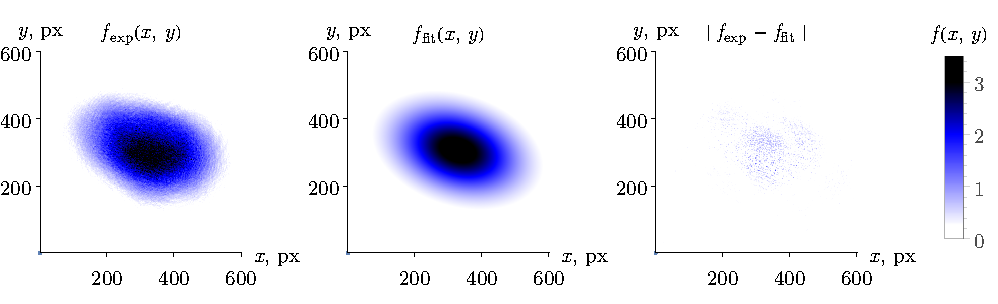
\includegraphics{figs/fit_mot_v2.pdf}
    \caption{Экспериментально сфотографированное распределение атомов $\sub{f}{exp}$, аппроксимация распределения атомов гауссовой функцией $\sub{f}{fit}$ \eqref{eq:photo_fit} и остатки аппроксимации $|\sub{f}{exp} - \sub{f}{fit}|$}
    \label{fig:fitmot}
\end{figure}

Далее распределение облака атомов аппроксимируется гауссовым распределением \cite{vlad, suk}, для нахождения полного числа атомов:
\begin{equation}
    \sub{f}{fit}(x, y) = B+A \exp\left(
        - \left(\frac{\tilde{x}}{\sigma_1}\right)^2 - \left(\frac{\tilde{y}}{\sigma_2}\right)^2
    \right),
    \hspace{10 mm} 
    \begin{pmatrix}
        \tilde{x} \\ \tilde{y}
    \end{pmatrix} = \begin{pmatrix}
        \cos \varphi & -\sin \varphi  \\
        \sin \varphi & \cos \varphi  \\
    \end{pmatrix} \begin{pmatrix}
        x-x_0 \\ y - y_0
    \end{pmatrix}.
    \label{eq:photo_fit}
\end{equation}
Учтен поворот облака в плоскости фотографирования на некоторый угол $\varphi$. 

\upar{Измерение количества атомов в МОЛ}
Полное число атомов тогда может быть найдено, как
\begin{equation}
    N = \pi A \sigma_1 \sigma_2.
\end{equation}
В случае, если лазерный пучок был выбран нерезонансным, то выражение для числа атомов $N$ с учётом \eqref{eq:deltaG} изменится к виду
\begin{equation}
    N = \frac{1}{\pi} \frac{\gamma}{\gamma^2+\delta^2} \pi A \sigma_1 \sigma_2,
\end{equation}
Основным влияющим фактором здесь является уширение резонанса по мощности $\gamma \to\gamma \sqrt{1+s}$, однако $\sub{s}{max} = \max (I / \sub{I}{sat}) \sim 0.2 \ll 1$, так что можем считать что $\gamma$ практически совпадает с шириной спектральной линии перехода 410.6 нм.



\upar{Измерение температуры атомов в МОЛ}
Наблюдение облака атомов, приведенного на рис. \ref{fig:fitmot}, происходит после выключения ловушки и разлёта атомов в течение некоторого времени. Остановимся подробнее на физике разлёта атомов. В начальный момент времени распределение атомов по скоростям соответсвует максвелловскому распределению, в коордиантном пространстве атомы можно считать нормально распределенными \cite{vlad}:
\begin{equation}
    f(\vc{r}, t) \propto \prod_{j=x,y,z} \int_{-\infty}^{+\infty} 
    \exp\left(
        - \frac{(r_i-v_j t)^2}{2 \sigma_j^2(0)} - \frac{m v_j^2}{2 \kB T}
    \right)
    \d v_j,
    \label{eq:MOTT}
\end{equation}
где $\sigma_j(t)$ соответсвует ширине облака атомов, $t$ -- время свободного разлёта, после выключения ловушки. Так как происходит свободное падение, то изменив систему отсчёта на свободно падающую вместе с облаком атомов, можем принебречь влияением гравитации. Интегрируя по скоростям \eqref{eq:MOTT}, находим искомую зависимость $\sigma_j(t)$:
\begin{equation*}
    f(\vc{r},t) \propto \prod_{j=x,y,z} \exp\left(
        - \frac{r_j^2}{2 \sigma_j(t)^2}
    \right),
    \hspace{10 mm} 
    \sigma_j(t)^2 =  \sigma_j^2(0) + \frac{\kB T}{m} t^2,
\end{equation*}
что позволяет по определенным из аппроксимации (рис. \ref{fig:fitmot}) фотографии данных нормальным распределением \eqref{eq:photo_fit}, определять температуру облака атомов в МОЛ. 



\begin{figure}[ht]
    \centering
    \subfigure[]{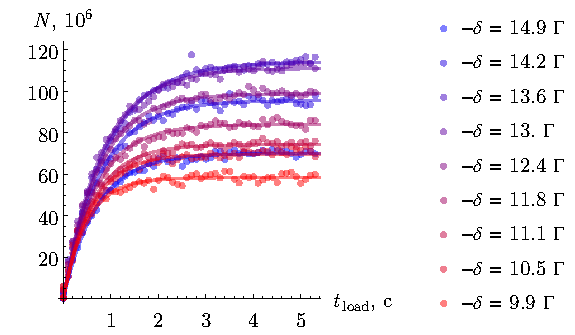
\includegraphics{figs/motload_v2.pdf}}
    \hspace{10 mm} 
    \subfigure[]{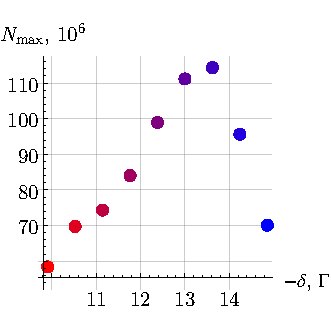
\includegraphics{figs/motload2_v2.pdf}}
    \caption{a) Динамика загрузки МОЛ для различных значений отстройки б)  Зависимость максимального числа атомов в МОЛ от величины отстройки $\delta$}
    % \label{fig:motload}
\end{figure}
